%
% This program is free software: you can redistribute it and/or modify
% it under the terms of the GNU General Public License as published by
% the Free Software Foundation, either version 3 of the License, or
% (at your option) any later version.

% This program is distributed in the hope that it will be useful,
% but WITHOUT ANY WARRANTY; without even the implied warranty of
% MERCHANTABILITY or FITNESS FOR A PARTICULAR PURPOSE.  See the
% GNU General Public License for more details.

% You should have received a copy of the GNU General Public License
% along with this program.  If not, see <http://www.gnu.org/licenses/>.

\documentclass{report}

\usepackage{mystyle}

\title{R 튜토리얼 \\ - Some R Problems Derived Me Nuts! -}
\author{iHELP Working Group \\ Chel Hee Lee \& Eugene Jung } 
\date{\today}

\begin{document}
\maketitle



\chapter{시작하면서}

통계소프트웨어 \texttt{R}을 사용하는데 이 문서가 도움이 되길 바랍니다. 
아래와 같은 내용에 중점을 두고자 하였습니다. 

\begin{itemize}
\item 원리중심의 문제해결을 설명하고자, 다양한 패키지들로부터 제공되는 함수들에 대한 사용법에 대한 설명은 가급적이면 피하려고 하였습니다.
따라서, 이 문서내에서는 특정 패키지가 해결할 수 있는 경우를 제외하고는 BASE (기본) 시스템을 이용하여 문제를 해결할 수 있도록 정리하려고 노력합니다.
\item 통계와 전산에 관련된 전문용어는 쉽게 풀어쓰거나, 용어에 대한 이해를 돕기 위한 참고 자료를 제공합니다. 
\end{itemize}

본 문서와 관련한 프로젝트의 시작일은 2010년 4월 10일이며, iHELP Working Group 관리자에 의하여 수시로 갱신되고 있습니다.
따라서, 이 문서는 어떤 특정한 기간을 두고 완성되으며, 오로지 업데이트된 버전만이 존재합니다.
만약, 이 문서를 읽고 있는 독자가 문서 내용에 대한 추가, 수정, 및 제안이 있다면 이를 \href{mailto:ihelp-urquestion@lists.r-forge.r-project.org}{ihelp-urquestion@lists.r-forge.r-project.org} 주소로 이메일을 보내주신다면 감사하겠습니다. 

아래와 명시된 분들의 도움이 없었다면 이 문서가 발전될 수 없었기에 그 감사의 말씀을 올리고 싶습니다. 
\begin{itemize}
\item 신종화 교수님 (서울종합과학대학원)
\end{itemize}

\paragraph{이 문서를 읽는 방법:} 
\begin{itemize}
\item ``완전초보에요''라는 챕터와 ``기초프로그래밍과 운영체제'' 챕터는 이 문서를 읽기 전에 반드시 먼저 읽으셔야 합니다.  
\end{itemize}

%%%%%%%%%%%%%%%%%%%%%%%%%%%%%%%%%%%%%%%%%%%%%%%%%%%%%%%%%%%%%%%%%%%%%%%%
%
%
%
%%%%%%%%%%%%%%%%%%%%%%%%%%%%%%%%%%%%%%%%%%%%%%%%%%%%%%%%%%%%%%%%%%%%%%%%

\chapter{완전 초보에요}

이 문서에서 ``초보''라는 의미는 아래에 나열된 사항들중 두 가지 이상에 해당되시는 분들을 의미합니다. 

\begin{itemize}
\item R 이라는 프로그래밍 언어 이전에 다른 프로그래밍 언어에 대한 경험이 전무하신 분,
\item 유닉스와 리눅스 시스템에 익숙하지 않으신 분,
\item 기초 통계 분석에 대한 도움이 필요하신 분,
\item 그냥 무엇을 해야할지 막막함에 쌓여 계신분 
\end{itemize}

이에 해당하시는 분들은 꼭 ``사용전 숙지사항'' 섹션을 꼭 읽어주시길 부탁드립니다.
R을 사용하시는데 있어 숙지사항의 내용을 기억하신다면, 매우 도움이 될 것입니다. 

\section{사용전 숙지사항}

초보라고 생각하시는 분들께서는 아래의 내용들에 대한 개념적 숙지해주시길 부탁드립니다.

\paragraph{데이터 입력과 처리:}  R 에서는 이용되는 모든 데이터들에 대한 처리는 열방향으로 이루어집니다.
이 말의 뜻은 데이터의 입력 및 변형, 그리고 연산에 사용되는 데이터들에 대한 처리순서는 열방향으로 나열된 후에 이루어지는 것을 말합니다. 
예를들어, 1부터 12까지 12개의 정수로 이루어진 수열 (즉, $\{ 1, 2, 3, 4, 5, 6, 7, 8, 9, 10, 11, 12 \}$)을 수학적인 표현으로 4행 3열의 행렬은 R은 아래와 같이 이해합니다. 

% 데이터 불러오기
% 보통 사람들은 R 콘솔에서 직접 입력한 데이터를 제외하고 그 외의 데이터는 *.txt, *.xlsx 이든 *.sav이든 모두 외부데이터로 생각하기
% 일쑤이다.
% 즉 foreign 팩키지를 사용해야 하는 경우를 제대로 구분하지 못한다. 그러니,
% > library(foreign)
% 을 선언할 줄 모르는 것은 당연하다.

% 그리고 인코딩이란 무엇인지를 모르는 사람은 보다 맞다.

\begin{Schunk}
\begin{Soutput}
1  5   9
2  6  10
3  7  11
4  8  12
\end{Soutput}
\end{Schunk}

따라서, 이 행렬에서 5라는 숫자값은 행렬의 1행 2열에 위치하고 있다고 할 수 있으며, 행렬의 5번째의 값이라고도 할 수 있습니다. 

\paragraph{대화식 사용과 결과를 보는 방법에 대해서:} R은 사용자가 주어지는 업무를 시키는 대로만 수행하는 유용한 프로그램일뿐, 그 이상의 내용은 수행하지 않는다는 점을 반드시 명심하셔야 합니다. 
따라서, R 프로그램을 시작하게 되면 아래와 같은 기호로 표시되는 프롬프트 (즉, 사용자의 명령어를 기다리는 기호)를 보여주게 됩니다. 
\begin{Schunk}
\begin{Soutput}
>
\end{Soutput}
\end{Schunk}

모든 명령어는 $>$ 기호 뒤에 작성하게 됩니다. 

가장 중요한 것은 분석자가 머릿속으로 상상하거나 기대하는 업무가 있다면, 분석자는 반드시 그 업무가 이루어지는 프로세스에 대해서 잘 알고 있어야 합니다.
따라서, R은 다른 통계 소프트웨어들과 같이 분석된 결과를 미리 보여주거나 혹은 분석이 된 모든 결과를 한 번에 다 보여주지 않습니다.
분석자가 확인하고자 하는 결과를 R에서 제공하는 함수를 통하여 중간 결과물들을 확인할 수 있습니다. 
우리는 분석자가 작업을 어떻게 진행하고 확인할 것인가에 대한 프로세스 차트를 먼저 작성한뒤 분석을 수행하기를 권장합니다.

\paragraph{통계분석의 절차:} 분석이라 것은 데이터에 대한 이해를 통하여 데이터가 가진 특징을 수학적 표현으로서 설명하기 위한 과정입니다. 
따라서, 데이터에 대한 직관적인 이해를 위해서 시각화 작업과 통계 모형이 요구하는 데이터 형식을 만드는 것이 중요합니다. 
이를 전처리 과정이라고 하며, 통계분석은 크게 아래와 같은 절차를 밟아 이루어집니다.

\begin{itemize}
\item 데이터 입출력과 클리닝, 그리고 분석 전처리 관련 테크닉들
\item 분석전 탐색적 시각화 작업 
\item 통계모형의 결정 및 적용 
\item 모형 적용 후의 보고서 생성 및 시각화 작업
\item 통계 모형 자체의 개발 또는 자동화 시스템 구축
\end{itemize}

따라서, 이 문서는 위에서 설명한 과정에 해당하는 순서대로 챕터들을 구성하였습니다. 

\paragraph{한글 표현과 인코딩에 관련하여:}

\texttt{R}은 한국어 사용자를 위한 한국어 인터페이스를 지원하고 있습니다. 
\textbf{그러나, 사용자는 이러한 한국어 지원이 단순히 사용자의 편의를 위한 선택적 사항이라는 점을 반드시 알고 있어야 합니다}.
또한, 분석시 본래의 정교한 표현은 번역된 한국어 보다는 원래의 영문이라는 점도 잊지 마셔야 합니다. 

현재 한국어에 관련된 작업은 UTF-8이라는 인코딩에 기반하여 한국어 품질관리 프로그램 (\url{http://ihelp.r-forge.r-project.org/lang_msg.html})을 통하여 이루어 지고 있으나, \texttt{R}을 한국어가 아닌 영문으로 설정하기 위해서는 다음의 주소를 눌러 그 내용을 확인해주시길 부탁드립니다. 
이 내용은 버전에 관계없이 일반적으로 통용되는 방법이나 윈도우즈 사용자에게 맞추어 작성되었습니다. 

\url{http://lists.r-forge.r-project.org/pipermail/ihelp-urquestion/2013-April/000003.html}

본래 데이터를 자국의 언어로 표현하는 방법은 UTF-8 이라는 인코딩을 이용하므로, 간혹 데이터가 올바르게 보이지 않을 경우가 있습니다. 
이러한 문제를 해결하기 위해서는 ``R을 지원하는 인코딩 중 올바르게 한국어를 표현해주는 코드를 찾는 방법'' (\url{http://lists.r-forge.r-project.org/pipermail/ihelp-urquestion/2013-April/000017.html}) 를 읽어보시길 바랍니다.

간혹, 잘못된 한글처리가 시스템 에러를 야기하는 경우가 있으므로, 이러한 경우에 한국어로 R을 사용하시는 분들께서는 다소 번거로우실지라도 보다 안정적이고 나은 R을 제공하기 위하여 그 내용을 \href{mailto:ihelp-urquestion@lists.r-forge.r-project.org}{ihelp-urquestion@lists.r-forge.r-project.org} 주소로 이메일을 보내주신다면 감사하겠습니다. 

단, 이러한 한글처리는 분석에 연관된 수치연산과는 아무런 관계가 없음을 반드시 알아주시길 부탁드립니다.


\paragraph{대소문자 구분에 관련하여:}
많은 분들이 이전에 SAS 소프트웨어를 사용하여 분석을 수행하셨을 것입니다.
SAS에서는 대소문자를 구분하지 않고 프로그램을 작성하게 되지만, R에서는 대소문자를 구분하므로 A 라는 변수와 a 라는 변수는 서로 다른 것임을 명심하시길 부탁드립니다. 


\paragraph{운영체제와 관련하여:}
R은 기본적으로 Unix (유닉스)와 같은 환경에서 작성되었습니다. 


\paragraph{패키지와 관련하여: }
R은 Add-on이라는 패키지 시스템을 이용합니다. 
이것은 기본 베이스 시스템에 추가로 필요한 기능들을 추가하는 의미입니다.
이러한 내용을 잘 모르는 상태에서 초보자가 가장 많이 겪는 실수는 어떤 함수를 사용하고자 할 때 ``xxx 함수가 없습니다'' 또는 ``xxx 함수를 찾을 수 없습니다''입니다.
이는 사용하고자 하는 함수가 R 기본 배포판에 포함되어 있지 않은 어떤 사용자에 의해서 제공된 특정한 패키지내에서 존재하기 때문입니다.
이런 경우에는 먼저 사용하고자 하는 함수가 어떤 패키지에 존재하는지 알아야 합니다.  
그리고, 해당 패키지를 설치했을 때에는 설치된 패키지를 사용할 수 있도록 로딩하는 과정을 거쳐야 합니다.

\begin{Schunk}
\begin{Soutput}
> library(pkg_name)	
\end{Soutput}
\end{Schunk}

패키지의 설치, 확인에 관련된 사항은 ``통계모형의 선택과 적용''이라는 챕터에 기록해두었습니다. 




\chapter{기초 프로그래밍과 운영체제}

우리는 독자가 R을 과학적 분석을 위해 필요한 일련의 프로세스를 진행하는 프로그래밍 언어로서 이해하기를 권장합니다.
이러한 프로세스를 수행함에 있어서 이 챕터에 있는 내용들을 먼저 숙지하시면 R을 사용하시는데 보다 수월함을 느끼시게 될 것입니다. 
따라서, 이 챕터에서는 원리 중심으로 R이 어떻게 동작하는가에 촛점을 맞추고 이들을 잘 활용할 수 있는 예제를 넣어 이해하는데 중점을 둘 것입니다. 

우리는 이러한 내용들을 설명하기 전에 에러와 경고에 대한 내용을 먼저 다룰 것입니다. 
알려져 있는 많은 교재들이 프로그래밍의 문법적 오류를 잡아내는 디버거라는 도구의 설명에 중점을 두고 있으나, 이 문서는 문법적 오류가 아닌 논리적 오류를 찾는 방법을 중심으로 내용을 전개할 것입니다. 
그 이유는 분석을 위한 프로그래밍은 논리적인 절차를 어떻게 잘 구성하는가에 따라서 그 효율성과 프로그램의 가독성이 달라지기 때문입니다. 

\section{에러에 관하여}

\subsection{에러의 정류와 관련 메시지}

\paragraph{문법적 오류}

\paragraph{논리적 오류}

\paragraph{오류와 경고의 다른점}

\paragraph{디버거를 사용하기전에}

분석작업에서는 주로 논리적 오류를 찾는것이 중요하지만, 패키지 개발에서는 디버거를 잘 다루는 기술적 요소가 더욱 요구됩니다. 
이러한 디버거의 사용에 대해서는 ``패키지 제작''이라는 챕터에서 다루도록 하겠습니다.

\subsection{에러 핸들링}
	만약, 메시지 역시 설명해줄려면  \texttt{stop()}, \texttt{warning()}도 함께 설명해주면 최고임.  
\paragraph{try()}

\paragraph{tryCatch()}

\begin{Schunk}
\begin{Soutput}
result <- tryCatch(
{
	수행하고자 하는 표현식
},
warning = function(w) {
	위에서 수행한 표현식이 경고를 발생시킬때 어떻게 처리하고자 하는지에 대한 표현식
},
error = function(e) {
	위에서 수행한 표현식이 에러를 발생시킬때 어떻게 처리하고자 하는지에 대한 표현식
}, finally {
	위에서 수행한 표현식에 대한 최종적 처리를 위한 표현식
}
\end{Soutput}
\end{Schunk}


\section{주석문의 사용}


\section{조건문:}
\texttt{repeat}, \texttt{while}에 대해서 간단히 보여주고, \texttt{break}과 \texttt{next} 를 알려주면 좋음. 


\paragraph{분기:}

\paragraph{switch}

\section{함수의 정의와 사용}

\paragraph{내장함수}

\paragraph{사용자 정의 함수}

\paragraph{do.call()}
% \item \texttt{do.call()} 함수를 사용하는 법에 대해서..
% http://cran.r-project.org/web/packages/rockchalk/vignettes/Rchaeology.pdf
% http://www.stat.berkeley.edu/classes/s133/all2011.pdf  (다운로드 해두었음 Desktop/tmpRsrc/all2011.pdf)
% http://www.stat.berkeley.edu/classes/s133/resources.html 

\paragraph{스코프}

\paragraph{인바이런먼트}

\section{벡터라이제이션과 반복문} 
\paragraph{반복문:}

\paragraph{벡터라이제이션:} \texttt{apply()}, \texttt{lapply()}, \texttt{sapply()}, \texttt{mapply()}의 사용방법


\section{객체와 속성}
\paragraph{속성:}
\paragraph{객체:}

\section{제네릭 함수와 클래스}
\paragraph{메소드:}
\paragraph{제네릭 함수:}
\paragraph{클래스:}

\section{스크립트 작성하기}
\paragraph{일괄처리}
\paragraph{실행하기}

\section{운영체제와 소통하기}
\paragraph{파일과 디렉토리 유틸리티}
\paragraph{시간과 관련된 명령어들}

	파일관리와 관계된 여러가지 유용한 유틸리티가 존재합니다. 
	\begin{itemize}
		\item \texttt{edit()},
		\item \texttt{file.edit()}
		\item \texttt{fix()}
		\item \texttt{file.show()}
		\item \texttt{file.path()}
		\item \texttt{list.files()}
		\item \texttt{dir.create()}
		\item \texttt{file.access()}
		\item \texttt{file.exists()}
		\item \texttt{file.copy()}
		\item \texttt{data.entry()}
		\item 너무 많아서 차근차근 예를들면서 하나씩 설명하겠습니다. 
	\end{itemize}

	
\section{프로그래밍 스타일 가이드}

%%%%%%%%%%%%%%%%%%%%%%%%%%%%%%%%%%%%%%%%%%%%%%%%%%%%%%%%%%%%%%%%%%%%%%%%%%%%%%%%%%%
%
%
%
%%%%%%%%%%%%%%%%%%%%%%%%%%%%%%%%%%%%%%%%%%%%%%%%%%%%%%%%%%%%%%%%%%%%%%%%%%%%%%%%%%%

\chapter{데이터 조작과 관련하여}

\section{데이터 파일 입출력}

데이터 입력과 출력은 R을 이용한 분석에서의 첫번째 단계와 마지막 단계라고도 할 수 있습니다. 
데이터가 입력된 형식은 매우 다양하지만,  일반적으로 R을 이용하여 데이터의 입출력을 하는데 있어 안전한 방법은 \texttt{.csv}이라는 파일확장자를 가진 파일을 이용하는 것입니다.
따라서, 가급적이면 다른종류의 파일확장자를 .csv로 먼저 변경한 뒤에 사용하는 것이 좋습니다. 

\subsection{입력}

\paragraph{다른 형식들: }

\subparagraph{고정형식}

\subparagraph{복잡한 구조를 읽어올때}

\subparagraph{.SAS}

\subparagraph{.SPSS}

\subparagraph{.URL}

\subparagraph{XML}

\subparagraph{.xls 또는 .xlsx}
마이크로소프트 엑셀을 사용합니다. 

\subparagraph{.csv}

\texttt{read.table()}이라는 함수를 아래와 같은 방법으로 이용하여 데이터를 읽어옵니다.

\begin{Schunk}
\begin{Soutput}
mydata <- read.table(file="./filename.csv", header=TRUE, sep=",")
\end{Soutput}
\end{Schunk}

여기에서 filename.csv 은 파일명입니다.

\subparagraph{입력과 관련된 문제해결법}

\texttt{read.table()} 함수를 이용하여 데이터를 불러오는데 있어서 많이 발생되는 오류는 ``데이터 파일을 작업디렉토리로부터 찾을 수 없다'' 또는 ``데이터 파일이 존재한 파일경로가 올바르지 않다'' 라는 것입니다. 

파일을 입력받을 때 R은 일반적으로 첫번째 인자에 주어진 파일명과 현재 작업디렉토리의 파일경로를 함께 묶어 절대경로를 생성한 뒤, 이 절대경로를 이용하여 파일명을 찾습니다. 
이러한 원리때문에 운영체제가 영어가 아닌 컴퓨터의 경우, 이 절대경로를 올바르게 생성하지 못할 경우가 있습니다. 
또한, 파일경로명에 띄어쓰기가 있는 경우 및 특수문자가 포함된 경우에 이러한 문제가 발생할 경우가 있습니다. 
따라서, 사용자는 간혹 문법에서 틀린 점도 없고, 불러오고자 하는 데이터 파일도 올바른 파일경로에 위치하고 있음에도 불구하고, 데이터를 찾을 수 없다는 에러 메시지를 보게 되는 경우가 있습니다. 
이러한 경우에 보다 안전한 방법으로 \texttt{read.table()} 사용하고자 한다면 아래와 같이 \texttt{file.choose()} 함수 또는 \texttt{file.path()} 함수를 이용하시길 바랍니다.

\begin{Schunk}
\begin{Soutput}
mydata <- read.table(file.choose(), header=TRUE, sep=",")
\end{Soutput}
\end{Schunk}

\texttt{file.choose()}는 탐색기를 띄워 사용자가 원하고자 하는 파일을 찾을 수 있도록 도와줍니다. 

\begin{Schunk}
\begin{Soutput}
mydata <- read.table(file.path(), header=TRUE, sep=",")
\end{Soutput}
\end{Schunk}

\texttt{file.path()}는 절대경로를 보다 안전하게 R이 이해할 수 있도록 도와줍니다. 


% http://www.statmethods.net/input/importingdata.html



\subsection{출력}


% R에서 편집한 데이터를 엑셀로 내보내는 방법[새로운 변수를 생성해서 기존 데이터에 더하려고 하는데
% (csv로 R에서 불러서 편집한 자료)]
% 
\paragraph{저장하기}
\subparagraph{.RData}
\subparagraph{.CSV}
\subparagraph{.HTML}
\subparagraph{.XML}

\subsection{메타데이터 처리}
\paragraph{원 데이터 소스에 데이터 구조 대한 이해와 데이터 엔트리: }

\paragraph{데이터셋 또는 변수에 주석첨가하기}


\section{데이터형에 대한 이해}

\subsection{벡터}

\subsection{행렬}

\subsection{데이터프레임}

\subsection{리스트}
\paragraph{리스트와 데이터 프레임 관계:}
% http://www.statmethods.net/input/datatypes.html
	\begin{Schunk}
	\begin{Soutput}
	ls()

	names(mydata)

	str(mydata)


	dim(object)

	class(obj)

	mydata

	head(mydata, n=10)

	tail(mydata, n=5) 

	length(obj)
	str(obj)
	class(obj)
	names(obj)
	
	c(obj,obj,...)
	cbind(obj, obj, ...)
	rbind(obj, obj, ...)
	
	obj
	
	ls()
	rm(obj)
	
	newobject <- edit(obj)
	fix(obj)
	\end{Soutput}
	\end{Schunk}
% 	levels(mydata$v1)

\subsection{배열}
\paragraph{배열과 행렬과 벡터와의 관계}

\subsection{결측치}

NA 와 NaN을 데이터로부터 찾고 싶어요. 
\texttt{is.na()}와 \texttt{is.nan()} 함수 사용법을 알려주면 좋음.  추가로 \texttt{is.null()}도 알려주면 \texttt{is}관련 함수들에 설명해주면 짱임.

\section{데이터 클리닝 및 전처리 테크닉}

\subsection{데이터셋에 관련하여}

\paragraph{변수명 변경하기}
\paragraph{조건에 부합하는 데이터셋 골라내기}
\paragraph{주어진 데이터셋으로부터 랜덤샘플 추출하기}
\paragraph{정렬하기}
\paragraph{데이터셋 합치기}
\paragraph{변수 추가 또는 제거}
\paragraph{종횡데이터를 횡형으로 변형하기}
\paragraph{횡형데이터를 종형으로 변형하기}
\paragraph{관측치의 개수 알아보기}
\paragraph{중복되는 값 찾아보기}
\paragraph{결측치에 대해서}

\subsection{문자형 변수들과 연관하여}

\paragraph{수치형 변수로 강제형변환 하기}
\paragraph{빈공간 모두 제거하기}
\paragraph{특정 문자열 뽑아내기}
\paragraph{변수의 길이 파악하기}
\paragraph{두 문자형 변수 결합하기}
\paragraph{대소문자 전환} 
\paragraph{요인과 관계하여}
\paragraph{라벨링 생성 및 변경하기}


\subsection{시간과 날짜에 관련하여}

\paragraph{날짜 데이터 생성}
\paragraph{년/월/일 따로 분리하기}
\paragraph{시간 데이터 생성}


\section{유용한 클리닝 테크닉들}

분석자가 보통 얻게 되는 데이터는 분석에 사용되는 통계모형에 적합한 경우는 드물기 때문에 분석자 스스로가 이러한 데이터를 형성하는 것은 필요한 기술중에 하나라고 할 수 있습니다.
% 

\paragraph{결측치를 바로 윗값으로 채워넣기: } 아래와 같이 주어진 데이터에 변수 ID는 결측값 없이 모든 값이 완전하게 잘 들어가 있는데, Week 변수에는 각 ID의 첫번째 레코드에만 해당하는 부분에 값이 들어가 있고 나머지부분에는 \texttt{NA}값이 들어가 있습니다. 

\begin{Schunk}
\begin{Soutput}
mydata <- data.frame(ID=c(rep(1,4), rep(2,4), rep(3,2)), Week=c(15, NA, NA, NA, 18, NA, NA, NA, 20, NA))

> mydata		

   ID Week
1   1   15
2   1   NA
3   1   NA
4   1   NA
5   2   18
6   2   NA
7   2   NA
8   2   NA
9   3   20
10  3   NA
\end{Soutput}
\end{Schunk}

이와 같은 데이터를 아래와 같이 자동으로 채워주려면 어떻게 해야 할까요? 	
	
\begin{Schunk}
\begin{Soutput}
   ID Week
1   1   15
2   1   15
3   1   15
4   1   15
5   2   18
6   2   18
7   2   18
8   2   18
9   3   20
10  3   20
\end{Soutput}
\end{Schunk}
	

이를 수행하는데에는 여러 가지 종류의 함수들이 다양한 패지키 안에 존재합니다.  
그러나, 이를 수행하는 기본 알고리즘은 동일하며, R 기본시스템만으로 작성이 가능합니다. 
아래의 함수를 복사하여 사용하시면 됩니다. 

\begin{Schunk}
	\begin{Soutput}
fill <- function(x, first, last){
	n <- last-first+1
	for(i in c(1:length(first))) x[first[i]:last[i]] <- rep(x[first[i]], n[i])
	return(x)
}
	\end{Soutput}
\end{Schunk}


\paragraph{각 아디이별로 첫번째와 마지막 레코드 찾아보기: } 위에서 주어진 데이터에서 ID 변수에서 보이는 것처럼 같은 관측치가 여러번 반복 측정되어 ID가 반복적으로 입력이 되었을 때, SAS에서처럼 각 아이디별로 첫번째와 마지막 레코드를 알수 있는 .FIRST 와 .LAST 같은 기능이 R에서는 어떻게 해야 하나요?

\begin{Schunk}
\begin{Soutput}
mydata$first <- !duplicated(mydata$ID)
mydata$last <- !duplicated(mydata$ID, fromLast=TRUE)		

> mydata
   ID Week first  last
1   1   15  TRUE FALSE
2   1   NA FALSE FALSE
3   1   NA FALSE FALSE
4   1   NA FALSE  TRUE
5   2   18  TRUE FALSE
6   2   NA FALSE FALSE
7   2   NA FALSE FALSE
8   2   NA FALSE  TRUE
9   3   20  TRUE FALSE
10  3   NA FALSE  TRUE
	\end{Soutput}	
\end{Schunk}

\paragraph{조건에 맞게 데이터 선택하기:} 데이터의 일부분만 골라 내고 싶어요.  예를들면, 위에서 사용된 예제에서 ID 가 1과 2인 데이터만 골라내고 싶다면 아래와 같이 할 수 있습니다. 

\begin{Schunk}
\begin{Soutput}
# 데이터 생성하기
mydata <- data.frame(ID=c(rep(1,4), rep(2,4), rep(3,2)), Week=c(15, NA, NA, NA, 18, NA, NA, NA, 20, NA))

# ID 변수에 있는 ID를 기준으로 첫번째와 마지막 레코드의 위치 알아내기 
idx.first <- which(!duplicated(mydata$ID))
idx.last <- which(!duplicated(mydata$ID, fromLast=TRUE))

# ID에 있는 NA값을 채워넣기 
mydata$Week <- fill(x=mydata$Week, first=idx.first, last=idx.last)

# 개별 ID에 대한 첫번째와 마지막 레코드에 대한 논리값을 추가하여 데이터 확장하기 
mydata$first <- !duplicated(mydata$ID)
mydata$last <- !duplicated(mydata$ID, fromLast=TRUE)

# 조건에 맞는 데이터 골라내기 
select <- subset(x=mydata, subset=(ID %in% c(1,2)))
> select
  ID Week first  last
1  1   15  TRUE FALSE
2  1   15 FALSE FALSE
3  1   15 FALSE FALSE
4  1   15 FALSE  TRUE
5  2   18  TRUE FALSE
6  2   18 FALSE FALSE
7  2   18 FALSE FALSE
8  2   18 FALSE  TRUE

# 추가적인 조건 부여하기
select.1 <- subset(x=mydata, subset=( (ID %in% c(1,2)) & first==TRUE ))
> select.1
  ID Week first  last
1  1   15  TRUE FALSE
5  2   18  TRUE FALSE
\end{Soutput}
\end{Schunk}


\paragraph{여러개의 엑셀시트로 구성된 엑셀파일 하나로 합치기:} 여러개의 엑셀시트로 구성되어 있는 엑셀파일을 불러와 하나의 데이터셋으로 합치기

\paragraph{리스트 중첩구조} 
가끔 리스트형으로 받아진 데이터가 중첩된 구조를 가지고 있어서, 한 번에 이를 불러오기를 해야할 때는 어떻게 해야할지.



%%%%%%%%%%%%%%%%%%%%%%%%%%%%%%%%%%%%%%%%%%%%%%%%%%%%%%%%%%%%%%%%%%%%%%%%%%%%%%%%%%%
%
%
%
%%%%%%%%%%%%%%%%%%%%%%%%%%%%%%%%%%%%%%%%%%%%%%%%%%%%%%%%%%%%%%%%%%%%%%%%%%%%%%%%%%%

\chapter{수학/확률/행렬/수치해석과 관련하여}

\section{수학함수들의 사용}
\paragraph{일반 수학함수들}
\paragraph{삼각함수들}
\paragraph{집합과 관련된 함수들}
\paragraph{기타 유용한 함수들}
% \item \texttt{which.max()}와 \texttt{which.min()}을 사용하는 방법 
\texttt{combn()} 함수를 이용하여 모든 조합을 찾기

\section{확률의 사용}

\subsection{밀도/누적 확률분포}

\paragraph{퍼센타일 값 찾기}

\subsection{표준 난수생성 함수}

\subsection{비표준 난수생성 알고리즘}
\paragraph{Multinomial random variables}

\paragraph{Correlated binary random variables}

\section{수치해석}

\subsection{미분}

\subsection{적분}
\paragraph{Laplace Approximation} 알고리즘을 구현하는 방법 -- 적분하는 방법에 많이 쓰임 (특히, 베이지안 컴퓨테이션) 

\subsection{최적화 문제}
\paragraph{Newton-Raphson} 알고리즘을 구현하는 방법 -- optimization 에 관련된 일종의 설명도 추가해주면 좋을 것 같음 


\section{행렬연산}
\paragraph{생성}

\paragraph{전치}

\paragraph{역행렬}

\paragraph{대각행렬}

\paragraph{기저값과 기저벡터}

\paragraph{행렬값}

\paragraph{행렬의 분해}


\section{시뮬레이션}
\subsection{Metropolis-Hastings} 알고리즘을 구현하는 프레임 워크 - 이것은 그냥 사용가능하게 바로 소스코드 붙여주기 (베이지안 컴퓨테이션에 많이 쓰임)

\subsection{Bootstrap} 
방법 -- 요건 아주 좋은 패키지가 있음 


%%%%%%%%%%%%%%%%%%%%%%%%%%%%%%%%%%%%%%%%%%%%%%%%%%%%%%%%%%%%%%%%%%%%%%%%%%%%%%%%%%%
%
%
%
%%%%%%%%%%%%%%%%%%%%%%%%%%%%%%%%%%%%%%%%%%%%%%%%%%%%%%%%%%%%%%%%%%%%%%%%%%%%%%%%%%%

\chapter{탐색적 데이터 분석}

여기에서 말하는 탐색적 분석이란 분석 초기에 단순히 데이터의 특징을 보는데 사용됩니다. 
또한, 이 과정은 데이터 클리닝과도 연관이 있습니다. 

\section{기술통계량 요약}

\paragraph{평균과 분산과 같은 기초요약 함수들}

\paragraph{그룹별 평균산출}

\paragraph{5분위수 구하기}

\paragraph{퀀타일}

\paragraph{표준화와 스케일링}

\paragraph{신뢰구간}

\section{분할표와 카이제곱 검정}

\section{z-검정}

\section{t-검정}

\section{}

%%%%%%%%%%%%%%%%%%%%%%%%%%%%%%%%%%%%%%%%%%%%%%%%%%%%%%%%%%%%%%%%%%%%%%%%%%%%%%%%%%%
%
%
%
%%%%%%%%%%%%%%%%%%%%%%%%%%%%%%%%%%%%%%%%%%%%%%%%%%%%%%%%%%%%%%%%%%%%%%%%%%%%%%%%%%%

\chapter{통계모형의 선택 및 적용}

각 섹션은 다음과 같은 방법으로 이루어져야 합니다. 
\begin{itemize}
\item 아래의 모형이 어느 경우에 사용되어야 하는가?
\item 모형을 사용하는데 있어서 요구되는 가정들은 무엇인가?
\item 모형의 계수에 대한 추정치는 어떻게 구하는가?
\item 모형의 진단
\item 추정치들에 대한 해석
\item 사용법들 
\item 모형에 대한 한계점
\end{itemize}

\section{분산분석 (Analysis of Variance-Covariance)}

\section{상관분석 (Correlation Analysis) }

\section{회귀분석 (Regression Analysis) }

\section{주성분분석 (Principle Component Analysis)}

\section{판별분석 (Discriminant Analysis) }

\section{군집분석 (Cluster Analysis) }

\section{시계열분석 (Time-Series Analysis) }

\section{일반선형모델 (GLM)}

\section{의사결정 나무(Decision Tree)}

\section{Longitudinal data analysis}

\section{생존분석 (Survivial analysis)}

\section{Mixture and latent class analysis}

\section{신경망 분석}

\section{기계학습 (Machine Learning)}

\section{메타 분석 (Meta Analysis)}


%%%%%%%%%%%%%%%%%%%%%%%%%%%%%%%%%%%%%%%%%%%%%%%%%%%%%%%%%%%%%%%%%%%%%%%%%%%%%%%%%%%
%
%
%
%%%%%%%%%%%%%%%%%%%%%%%%%%%%%%%%%%%%%%%%%%%%%%%%%%%%%%%%%%%%%%%%%%%%%%%%%%%%%%%%%%%

\section{패키지 관리}
\begin{enumerate}
\item 	이와 반대로 현재 연결된 라이브러리를 떼어낼 수도 있습니다. 

	\begin{Schunk}
	\begin{Soutput}
	> detach(package:pkg_name)	
	\end{Soutput}
	\end{Schunk}

	% 웹에 > detach(package:pkg_name) 과 5. 패키지를 설치 (분류: 사용자 환경)이 한 줄 띄어져야 함.

	\item 패키지를 설치 (분류: 사용자 환경)  
	
	\textsf{(답변)} 설치되는 패키지의 \textbf{설치위치}와 \textbf{의존성}에 대해서 반드시 알아야 합니다. 
	
	\begin{Schunk}
	\begin{Soutput}
	> install.packages("패키지명", dependencies=TRUE, )
	\end{Soutput}
	\end{Schunk}
% 을 쓰지 못하는 사례도 허다하다. package를 설치할 때 메뉴에서 [패키지 -> 패키지 설치하기]를 선택하고 난 뒤
% [mirror]를 선택한 뒤 패키지 리스트에서 하나씩 어디선가 본 패키지 이름을 어렵게 어렵게 찾아 더블클릭하는 절차를 따르는 것이다.

	\item 설치된 패키지의 목록을 확인하는 방법을 알고 싶습니다.
\end{enumerate}


%%%%%%%%%%%%%%%%%%%%%%%%%%%%%%%%%%%%%%%%%%%%%%%%%%%%%%%%%%%%%%%%%%%%%%%%
%
% Visualization
%
%%%%%%%%%%%%%%%%%%%%%%%%%%%%%%%%%%%%%%%%%%%%%%%%%%%%%%%%%%%%%%%%%%%%%%%%

\chapter{비쥬얼라이제이션}

\section{플랏 커스터마이징}
\paragraph{포인트와 텍스트 사이즈 변경}
\paragraph{마진 조절하기}
\paragraph{한페이지에 다중 그래프 생성}
\paragraph{축 라벨, 보조선 조절하기}
\paragraph{선의 종류와 너비조절}
\paragraph{색상에 대해서}


\section{그래픽 요소 추가하기}
\paragraph{직선 넣기}
\paragraph{플랏 기호 변경}
\paragraph{다중 플랏 보여주기}
\paragraph{제목/부제목 수정}
\paragraph{라벨 붙이기}
\paragraph{레전드 넣기}
\paragraph{수학기호 표현하기}
\paragraph{텍스트 집어넣기}

\section{그래픽 출력하기}
\paragraph{Postscript}
\paragraph{PDF}
\paragraph{JPEG, TIFF, PNG}

\section{플랏팅의 종류}

\subsection{산점도}
\subsection{바플랏}
\paragraph{다중 바플랏}
\subsection{히스토그램}
\subsection{줄기-잎 그림}
\subsection{Q-Q 플랏}
\subsection{3차원 플랏}



\begin{enumerate}

\item \texttt{coordinating system}을 활용하기

\item \texttt{Lattice} 패키지를 이용하여 아래와 같은 그림을 생성해보기 (가장 단순한 예제임 - 팁 보다는 튜토리얼 형식으로?)

%\rotatebox{-90}{\includegraphics{./lattice_ex1.eps}}
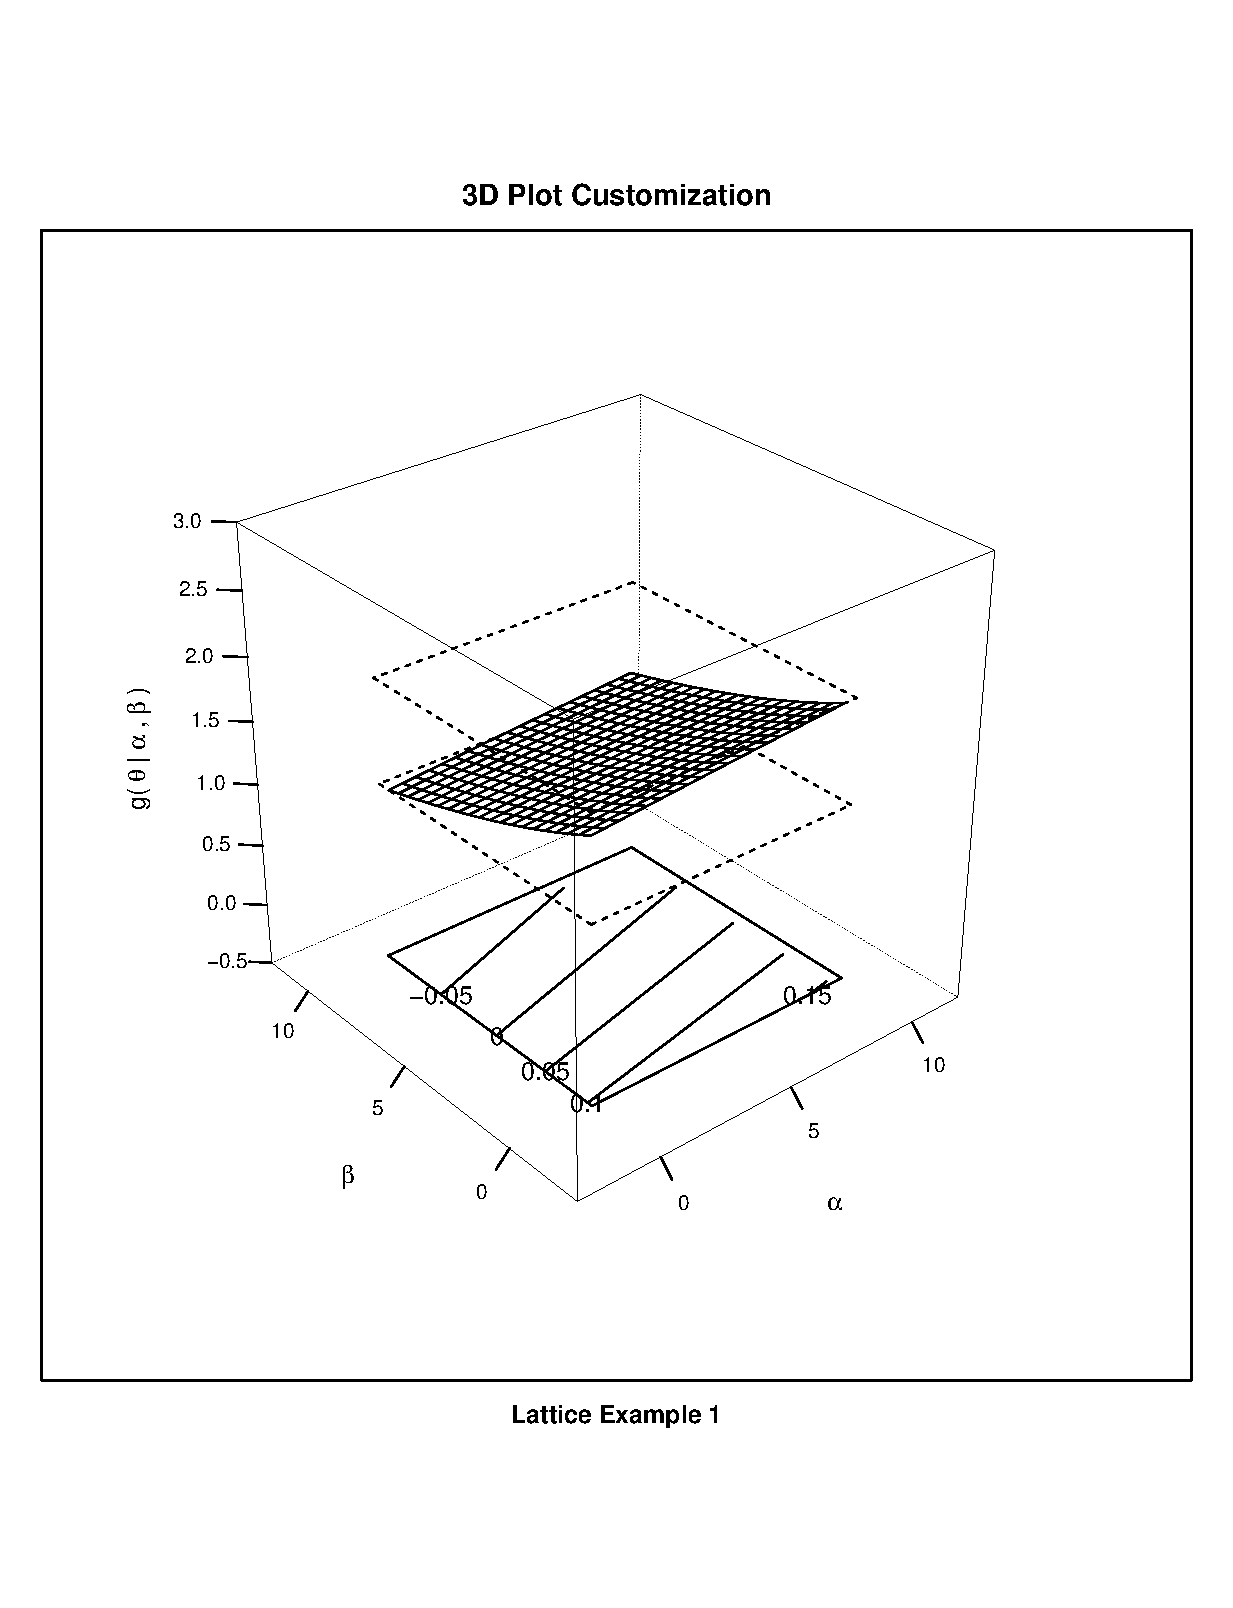
\includegraphics{./img/lattice-fig.eps}


\item \LaTeX 의 문서에 포함될 \texttt{.eps} 그래픽을 \texttt{R}에서 뽑았을 때는 아무런 문제가 없어 보였는데, 정작 \texttt{pdf}로 문서를 뽑아 보니까 이 그래픽이 들어간 페이지가 90도로 돌아가 있거나 혹은 그래픽이 90도로 회전되어 있을 경우에는 아래와 같이 하면 됩니다.

\begin{Schunk}
 \begin{Sinput}
  postscript(file=``filename.eps'', onefile=FALSE, horizontal=FALSE)
 \end{Sinput}
\end{Schunk}

이 문제에 대한 출처는 \texttt{postscript} 도움말입니다.

이문제를 다른 방법으로도 해결할 수 있습니다.  (대충 서너개 더 있음).

\item 새로운 그래픽 객체를 생성하는 방법을 설명해줘서 사용자가 추후에 독립적인 그래픽을 생성할 수 있게 도와주기 


	\item (접수: 2013-APR-23)  저는 다각형을 그리고 싶습니다. 
	
	\textsf{(답변)}  이것은 간단히 2차원-랜덤포인트 생성한 뒤에 \texttt{polygon()} 함수를 써서 보여주면 됨. 

\end{enumerate}

% ggplot2에서 stat_density2d에 오류가 있는것 같습니다. 모든 경우에 NA가 return된다는 보고




%%%%%%%%%%%%%%%%%%%%%%%%%%%%%%%%%%%%%%%%%%%%%%%%%%%%%%%%%%%%%%%%%%%%%%%%
%
% Utilities
%
%%%%%%%%%%%%%%%%%%%%%%%%%%%%%%%%%%%%%%%%%%%%%%%%%%%%%%%%%%%%%%%%%%%%%%%%



\chapter{분석 후 개발과 관련하여}
\section{클래스와 메소드 그리고 패키지 제작}
\begin{enumerate}
\item 패키지를 만들고 싶어요. (흠.. Generalized Linear Model 프레임워크 흉내내서 똑같이 만들어보기 실습자료로 제공해주기)
\end{enumerate}



%%%%%%%%%%%%%%%%%%%%%%%%%%%%%%%%%%%%%%%%%%%%%%%%%%%%%%%%%%%%%%%%%%%%%%%%
%
% Miscellinous
%
%%%%%%%%%%%%%%%%%%%%%%%%%%%%%%%%%%%%%%%%%%%%%%%%%%%%%%%%%%%%%%%%%%%%%%%%


%%%%%%%%%%%%%%%%%%%%%%%%%%%%%%%%%%%%%%%%%%%%%%%%%%%%%%%%%%%%%%%%%%%%%%%%
%
%
%
%%%%%%%%%%%%%%%%%%%%%%%%%%%%%%%%%%%%%%%%%%%%%%%%%%%%%%%%%%%%%%%%%%%%%%%%

\section{간단한 GUI 제작 해보기}

\begin{enumerate}
	\item 다른 언어로 인터페이싱 하는 방법마로, 그냥 \texttt{R}에서 주어지는 패키지를 이용해서 간단한 GUI 환경만들기
	\item 아마도... R Commander를 확장하는 방법을 예로 들면 좋을 것 같음
	\item 원리도 간단히 설명해주면 더욱 좋을 것 같음. 
\end{enumerate}


%%%%%%%%%%%%%%%%%%%%%%%%%%%%%%%%%%%%%%%%%%%%%%%%%%%%%%%%%%%%%%%%%%%%%%%%
%
%
%
%%%%%%%%%%%%%%%%%%%%%%%%%%%%%%%%%%%%%%%%%%%%%%%%%%%%%%%%%%%%%%%%%%%%%%%%


\chapter{미분류 질문들}

% 콘솔 컨트롤
% ctrl + L을 누르면 콘솔의 내용이 모두 지워짐

이 섹션에 등록된 질문들은 접수만 되고 아직은 답변되지 않은 상태입니다
% http://www.columbia.edu/~cjd11/charles_dimaggio/DIRE/resources/R/rFunctionsList.pdf
% http://www.ats.ucla.edu/stat/r/library/advanced_function_r.htm
% http://www.sr.bham.ac.uk/~ajrs/R/r-function_list.html
% http://www.scidav.org/techno/r_environments


% 이런 느낌은 특히 최소한 내가 알기로는 경영학과 경제학 분야(거의 확실함) 및 사회학, 심리학 분야가 특히 심하다. 
% 그리고 이들 분야에서는
% R의 다양한 기능(특히 visualization) 또는 packages를 필요로 하지 않을 가능성이 높다. 왜냐하면 분석 방법이 단순하기 때문이다.
% 여기에서 분석 방법이 단순하다는 것은 그 이론적 배경이 쉽다는 것을 의미하는 것이 아니라 절차상의 얘기이다.
% 언급한 분야에서 학술연구에서 실행되는 분석의 양을 보면 대부분 [기술통계 - 상관관계 - 차이분석, 회귀분석, 구조방정식분석] 정도로
% 분석이 마무리 되기 때문이다. 그리고 대부분 표(table)로 결과를 보고하는 형식을 따르고 있다.
% 분석 모형 자체를 다루는 연구가 거의 없는 것이다. 따라서 R의 작업 방식은 그들에게는 불필요할 지도 모른다.

% 그러나 여전히 R의 다양한 source를 필요로 하는 아주 작은 규모의 학술연구 분야는 존재한다. 따라서 여기의 tips에는 이들을 고려하여
% R 사용에 도움이 될 만한 사항들을 정리하고자 한다.
% 개인적으로는 통계학 및 다른 분야의 연구 과정이 어떻게 진행되는지 잘 모르는 것도 한 몫하여 이에 해당하는 부분은 다른 이의 도움이
% 절실하다.

% 덧붙여 나는 윈도우 환경에서의 R tip에 주목하고자 한다(Mac이나 유닉스/리눅스 환경에서의 R 사용에 관한 tip도 다른 이의 도움이 필요한
% 부분이다). 그 이유는 내가 윈도우에서 SPSS와 SAS를 숙련시켜 왔기 때문에 대부분의 통계분석 초심자들도 윈도우 환경에서 R 을 접하게
% 될 것이라는 막연한 억측 때문이다. 시간이 지나면서 여러 사람들을 만나보게 꼭 그렇지만은 않다는 것을 알게 되었지만 최소한 경영학과
% 경제학 분야에 속한 사람들은 그럴 것이라는 확신 때문이다. 이것은 다른 분야의 사람들을 홀대하는 것이 아니라 나의 능력의 한계 때문이다.
% 실제로 나의 경우에도 최근에 C 언어, CentOS, 그리고 MySQL도 공부하기 시작했으니 오해는 하지 말기 바란다(누군가는 포기하라고도 했다.
% 왜냐하면 지금 그것들을 공부하기에는 분량이 너무 많고 난이도가 낮지 않기 때문이다). 그런데 결국에는 내 전공분야에서의 R 사용은
% 그 분량이 많지 않고 리눅스/유닉스 기반의 R 사용에 보다 많은 시간과 지면을 할애하게 될 것이라는 생각이 든다.

% R은 최근의 빅데이터라는 화두와 함께 큰 주목을 받고 있다. 하지만 대부분의 사람들, 특히 사회과학 전공자들은 이 개념적 정의도 제대로
% 알지 못하며 들어보지 못한  전문용어(SQL, Hadoop, 그리고 Mapreduce 등)에 혹하고 있는 실정이다.
% 나의 경우 R을 구글링(googling)으로 공부하였다. 왜냐하면 내가 재학하던 대학에서는 R 교육 프로그램이 없었기 때문이다. 처음 접하게 된
% 것은 미시경제분석 수업이었다. 그 수업에서 교수님이 수업을 진행하시는데 R을 사용한 것이다(SAS도 조금 사용했었으나 SPSS 는 잡동사니
% 취급을 하셨던 것으로 기억한다). 누군가에게 강의를 받는 식의 교육은 그것이 전부였다. 이후의 학습은 모두 맨땅에 해딩과 계란으로
% 바위깨기 식이었다. 이 R tips 과정은 이러한 어려움을 덜어주기 위한 방안이 될 수도 있을 것이다.
% 그러기를 한참 후 어느 정도 익숙해지고 나니, 또 연구자로서의 건방이 살아나 R 교육이 어떻게 이루어지고 있는 지가 궁금해졌다.
% 이 부분은 나중에 다시 써 볼라오,,,


\begin{enumerate}
	
% 아래의 주소로부터 질문 다 만들어내기 	
% http://www.statmethods.net/input/valuelabels.html


	\item (접수: 2013-APR-23)  제가 가진 데이터셋이 있는데, 이 데이터를 어떤 특정한 변수들의 값을 이용하여 분류하려고 합니다.  어떻게 해야하나요?
	
	\textsf{(답변)}  요것은 \texttt{split()} 함수를 이용하도록 알려줄 것. 

	\item (접수: 2013-APR-23) 제가 가진 데이터 프레임에 NA 값들이 있는데, NA 때문에 분석이 이상해지는 것 같아, NA를 가진 데이터 행자체를 없애고 싶습니다.  한번에 해주는게 없나요? 
	
	\textsf{(답변)}  요건 \texttt{na.omit()}과 같은 함수를 이용하는 법을 알려줄 것.  흠.. \texttt{na.action}이라는 개념을 알려주면 더욱 좋음. 

	\item (접수: 2013-APR-23) 논리형 벡터가 있는데, 이 벡터의 구성요소가 모두 TRUE 인지 알고 싶습니다. 
	
	\textsf{(답변)} 이건 \texttt{isTRUE()}함수와 \texttt{all()}함수를 통해 알려주면 매우 좋음.
		
	\item (접수: 2013-APR-22) 선형방정식 $AX=b$의 해 $X$를 찾으려면 어떻게 해야 하나요? 
	
	\textsf{(답변)} \texttt{solve()} 함수의 사용법을 알려줄 것.
	
	\item (접수: 2013-APR-21) R 패키지를 CRAN에 올리는 방법을 알려주세요 
	
	\textsf{(답변)} 이 질문을 대답할 때는 반드시 CRAN Package Submission Guideline에 대해서 알려줘야 함.  (이거 번역해 놨는데 당췌 어디에 뒀는지 찾을 수가 없음, 2013-04-20 까지 못 찾으면 새로이 번역할 것)
	
	\item (접수: 2013-APR-19) R은 처음부터 기존의 통계팩키지와는 다른 모습에 약간 두렵기까지 합니다.  기존의 분석은 일반적으로 $[$프로그램 실행 $->$ 데이터 불러오기 $->$ 분석(메뉴클릭:SPSS 또는 명령어입력:SAS) $->$ 실행$]$의 절차를 밟아 왔기에 모든 결과를 한 번에 보여주는 식입니다. 그러나 R은 그렇지 않아 이러한 점부터 생소하고 이상합니다.  데이터를 불러오기 하면 바로 데이터시트를 볼 수 있는 것도 아닙니다 (접수날짜: 2013-APR-17).

	\item (접수: 2013-04-18, Reproducibility=NO) read.xlsx함수를 이용해 xlsx파일에서 데이터프레임형태로 가져옵니다. 이 때 [3,3] 셀에 있는 텍스트가 "3월" 이라고 할 때 temp[3,3] == "3월" 이렇게 비교하려고 하면 제대로 비교가 안되더군요.. 한글 텍스트로 이루어진 변수값를 비교하는 방법이 어떤게 있는지 궁금합니다.
	
	\item 분석을 하고 나면 결과를 그래프나 그림으로 나타내게 되는데 R에서는 그림을 나타내는 창이 하나만 나타나서 동시에 두 개를 보지 못하는 경우가 허다한데, 이의 해결방법은 없나요? (접수: 2013-APR-13, 분류: 그래픽스 관련) 
	
	\textsf{(답변)} \texttt{R}에서는 그래픽 디바이스가 그래픽 생성시 마다 초기화되어 다시 보여줌으로서 그래픽 창이 하나만 계속 보여지는 것입니다.  새로운 그래프를 또다른 장치를 통해 보여주고자 한다면 \texttt{X11()}이라는 명령어를 이용하면 됩니다.  
	이 명령어는 유닉스환경에 설치된 \texttt{R}의 경우에 해당합니다.  
	


\end{enumerate}


\section{답변되지 않을 수도 있는 질문들}

\begin{enumerate}
	\item (접수: 2013-04-18, Reproducibility=NA) R의 장점이자 단점이라고 생각되는 것 중에 하나가 엄청난 수의 패키지들임. 즉 어떤 분석을 하고자 할 때 그것에 대해 하나의 패키지가 있는 것이 아니라 대체적으로 사용가능한 패키지들이 존재하는데 이들 중 어느 것을 써야할 지 잘 모름. 다른 분석 프로그램의 경우 이러한 문제가 없는데... 결국엔 어떻게 제일 성능이 좋은? 결과가 신뢰할 만한? 좋은 패키지를 선택하는가를 알려주었으면 좋겠씀돠.
	
	\textsf{(답변)} 이것은 경험에 해당되며, 해당분야의 전문가로부터의 조언을 받는 것이 안전합니다.  그렇지 않다면, 직접 베이스를 이용하여 작성하면 됩니다. 
	
\end{enumerate}
\end{document}

% R을 사용해서 web 크롤링을 하는데 속도가 엄청 느리네요 scan() 함수를 쓰면 url로부터 html데이터를 받게 되는데 이것을 substring()함수와 regexprs()함수를 사용하여 적절히 데이터를 분해 하는 작업을 하는데 엄청느리네요. 원체느린거 같은데 혹시 해결방안 아시는분 게시나요?

% R에 있는 ggplot2 패키지를 이용해 얻은 얻은 plot그림을 웹에 보여주는 방법에 대해 아시는 분 계신가요?
 
